\documentclass[11pt,a4paper]{article}

% ── packages ──────────────────────────────────────────────────────────────────
\usepackage{amsmath,amssymb,amsthm}
\usepackage{geometry}
\usepackage{booktabs}
\usepackage{array}
\usepackage{hyperref}
\usepackage{tikz}
\usepackage{pgfplots}
\pgfplotsset{compat=1.18}
\usetikzlibrary{arrows.meta,positioning,calc}

\geometry{margin=2.5cm}

% ── theorem-like environments ─────────────────────────────────────────────────
\newtheorem{remark}{Remark}
\newtheorem{proposition}{Proposition}

% ── custom commands ───────────────────────────────────────────────────────────
\newcommand{\N}{\mathcal{N}}
\newcommand{\LN}{\operatorname{LogN}}
\newcommand{\dif}{\,\mathrm{d}}
\newcommand{\E}{\mathbb{E}}
\newcommand{\R}{\mathbb{R}}
\newcommand{\Rp}{\mathbb{R}_{+}}
% use \phi for standard normal pdf (amsmath already defines \varphi)

% ── title ─────────────────────────────────────────────────────────────────────
\title{Converting Between Gaussian and Lognormal Families\\[4pt]
       \large Two strategies --- a bridge to Girsanov\\[4pt]
       \normalsize Version~6}
\date{2026}
\author{}

% ══════════════════════════════════════════════════════════════════════════════
\begin{document}
\maketitle
\tableofcontents
\bigskip

% ══════════════════════════════════════════════════════════════════════════════
\section{The program}
\label{sec:program}

Our ultimate goal is to understand how geometric Brownian motion (GBM) is converted into a
martingale under the risk-neutral measure --- the core of Black--Scholes.  That conversion is an
instance of Girsanov's theorem, which operates on infinite-dimensional path space and is
technically demanding.

The strategy here is to build intuition through finite-dimensional analogues first, working
through two families of distributions and two conversion strategies before lifting to processes.
Each step will reappear, in more complex form, in the Girsanov argument.

Recall the two strategies (from the companion notes):

\medskip
\begin{center}
\begin{tabular}{lll}
\toprule
\textbf{Strategy} & \textbf{Action} & \textbf{Keeps fixed} \\
\midrule
Way~1 & Change the measure on source space $\Omega$ & the map $f:\Omega\to\R$ \\
Way~2 & Change the map $f\to g$                    & the measure on $\Omega$ \\
\bottomrule
\end{tabular}
\end{center}
\medskip

\noindent\textbf{The simplest setting: $\Omega=\R$.}
When $\Omega=\R$ and $f=\mathrm{id}$, Way~1 means replacing
$\mu_1=\N(\mu_1,\sigma_1^2)$ directly with a reweighted version on $\R$.
On $\Omega=\R$ we have explicit control over the measure.

We work through four cases in order:
\medskip
\begin{center}
\begin{tabular}{lll}
\toprule
\textbf{Section} & \textbf{Source} & \textbf{Target} \\
\midrule
\S\ref{sec:normal-way2} & $\N(\mu_1,\sigma_1^2)$ & $\N(\mu_2,\sigma_2^2)$ via Way~2 (affine map) \\
\S\ref{sec:normal-way1} & $\N(\mu_1,\sigma_1^2)$ & $\N(\mu_2,\sigma_2^2)$ via Way~1 (reweight) \\
\S\ref{sec:logn-way2}   & $\LN(\mu_1,\sigma_1^2)$ & $\LN(\mu_2,\sigma_2^2)$ via Way~2 (power map) \\
\S\ref{sec:logn-way1}   & $\LN(\mu_1,\sigma_1^2)$ & $\LN(\mu_2,\sigma_2^2)$ via Way~1 (reweight) \\
\bottomrule
\end{tabular}
\end{center}

% ══════════════════════════════════════════════════════════════════════════════
\section{Normal family, Way~2: the affine map}
\label{sec:normal-way2}

\subsection{The map}

Let $\Omega=\R$, $\mu_1=\N(\mu_1,\sigma_1^2)$ on $\Omega$, and $f_1=\mathrm{id}$, so the
induced measure on $B=\R$ is $\nu_1=\N(\mu_1,\sigma_1^2)$.

We want $\nu_2=\N(\mu_2,\sigma_2^2)$ on $B$.  As discussed in the companion notes, this is
achieved by a map $g:B\to B$ on the target, with $f_2=g\circ f_1=g$.

The standard normal $Z\sim\N(0,1)$ satisfies $\mu_1+\sigma_1 Z\sim\N(\mu_1,\sigma_1^2)$ and
$\mu_2+\sigma_2 Z\sim\N(\mu_2,\sigma_2^2)$.
So we need a map sending $\mu_1+\sigma_1 z\mapsto\mu_2+\sigma_2 z$.
Solving: $z=(y-\mu_1)/\sigma_1$, so the map is
\[
  g(y)=\mu_2+\frac{\sigma_2}{\sigma_1}(y-\mu_1),
\]
an affine map: scale by $\sigma_2/\sigma_1$ around $\mu_1$, then shift to $\mu_2$.

\subsection{Verification by change of variables}

$g$ is strictly increasing with $g'(y)=\sigma_2/\sigma_1$ and
$g^{-1}(y)=\mu_1+\frac{\sigma_1}{\sigma_2}(y-\mu_2)$.  The pushforward density (Form~A):
\[
  f_{\nu_2}(y)
  =f_{\nu_1}(g^{-1}(y))\cdot\frac{1}{|g'(g^{-1}(y))|}
  =\frac{1}{\sigma_1}\phi\!\left(\frac{g^{-1}(y)-\mu_1}{\sigma_1}\right)\cdot\frac{\sigma_1}{\sigma_2}
  =\frac{1}{\sigma_2}\phi\!\left(\frac{y-\mu_2}{\sigma_2}\right),
\]
which is the $\N(\mu_2,\sigma_2^2)$ density. \checkmark

\subsection{Special cases}

\begin{center}
\begin{tabular}{lll}
\toprule
\textbf{Case} & \textbf{Map }$g(y)$ & \textbf{Effect} \\
\midrule
$\sigma_1=\sigma_2,\;\mu_1\ne\mu_2$ & $y+(\mu_2-\mu_1)$ & pure shift \\
$\mu_1=\mu_2,\;\sigma_1\ne\sigma_2$  & $\mu_1+\dfrac{\sigma_2}{\sigma_1}(y-\mu_1)$ & scale around mean \\
$\mu_1=0,\;\sigma_1=1$ (standard)   & $\mu_2+\sigma_2 y$ & the standard parameterisation \\
\bottomrule
\end{tabular}
\end{center}

% ─────────────────────────────────────────────────────────────────────────────
\subsection{The affine group and its inversion operator}
\label{sec:affine-group}

The normal-to-normal map is most cleanly understood through the group of affine functions
on~$\R$.

\medskip\noindent\textbf{The affine family.}
Define
\[
  \mathrm{Af} = \bigl\{f:\R\to\R \mid f \text{ is affine}\bigr\}
             = \bigl\{\,\mathrm{af}_{a,b}(x) = a + bx \;\bigm|\; a,b\in\R\bigr\}.
\]
$\mathrm{Af}$ is closed under composition:
$\mathrm{af}_{a_2,b_2}\circ\mathrm{af}_{a_1,b_1}=\mathrm{af}_{a_2+b_2 a_1,\,b_2 b_1}$.
A map $\mathrm{af}_{a,b}$ is invertible if and only if $b\ne 0$, in which case
\[
  y = a + bx
  \;\Longrightarrow\;
  x = \frac{y-a}{b} = -\frac{a}{b} + \frac{1}{b}\,y
  = \mathrm{af}_{-a/b,\;1/b}(y).
\]

\medskip\noindent\textbf{The coefficient operator for inversion.}
The passage from a function to its inverse corresponds to a map on the parameter pairs
$(a,b)$.  Define the \emph{coefficient operator}
\[
  \boxed{C:\;(a,b)\mapsto\!\left(-\frac{a}{b},\;\frac{1}{b}\right)},
  \qquad
  C:\R\times\R\setminus\{0\}\;\longrightarrow\;\R\times\R\setminus\{0\}.
\]
Then $(\mathrm{af}_{a,b})^{-1}=\mathrm{af}_{C(a,b)}$.

\noindent\textbf{Verification.}  $C$ is an involution: $C(C(a,b))=C(-a/b,1/b)=
(-(-a/b)/(1/b),\,b)=(a,b)$.  This reflects the fact that inverting twice returns the
original map. \checkmark

% ─────────────────────────────────────────────────────────────────────────────
\subsection{How $C$ acts on lines in parameter space}
\label{sec:C-geometry}

Every affine map $\mathrm{af}_{a,b}$ corresponds to a point $(a,b)$ in the parameter plane
$\R\times(\R\setminus\{0\})$.  Families of affine maps that share a structural
constraint correspond to \emph{curves} in this plane.  The operator $C$ acts on the whole
plane, and it is illuminating to track what it does to the most natural curves: lines.

\medskip\noindent\textbf{Three canonical line families and their images under $C$.}

Let $(u,v) = C(a,b) = (-a/b,\;1/b)$.  Three families of lines in $(a,b)$-space and their
$C$-images in $(u,v)$-space:

\begin{center}
\renewcommand{\arraystretch}{1.6}
\begin{tabular}{p{3.8cm}p{3.2cm}p{4cm}p{3cm}}
\toprule
\textbf{Family in $(a,b)$} & \textbf{Condition} & \textbf{Image under $C$} & \textbf{Type} \\
\midrule
Horizontal: $b = c$
  & $b$ fixed, $a$ free
  & $v = 1/c$ \newline(horizontal line)
  & horiz.\ $\to$ horiz. \\
Ray through origin: $a = \lambda b$
  & slope $\lambda$, $a/b=\lambda$
  & $u = -\lambda$ \newline(vertical line)
  & ray $\to$ vertical \\
Vertical: $a = c$
  & $a$ fixed, $b$ free
  & $u = -cv$ \newline(ray through $0$)
  & vertical $\to$ ray \\
\bottomrule
\end{tabular}
\end{center}

\noindent Note the duality: $C$ swaps ``vertical lines'' with ``rays through the origin'',
and maps horizontal lines to horizontal lines (at the reciprocal height).  This is a
consequence of the involution property $C^2=\mathrm{id}$.

\bigskip

The two plots below show the three families before and after applying $C$.  Each coloured
line in the left panel maps to the correspondingly coloured curve/line in the right panel.

\bigskip
\begin{center}
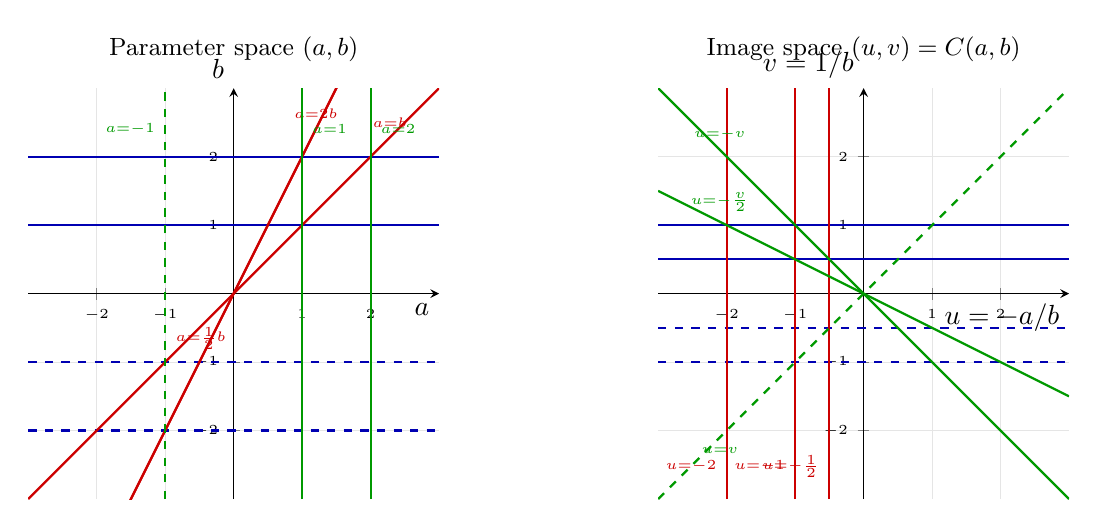
\begin{tikzpicture}
%% LEFT PANEL: lines in (a,b) parameter space
\begin{scope}
\begin{axis}[
  name=left,
  width=6.8cm, height=6.8cm,
  xmin=-3, xmax=3, ymin=-3, ymax=3,
  axis lines=center,
  xlabel={$a$}, ylabel={$b$},
  xlabel style={anchor=north east},
  ylabel style={anchor=south east},
  title={\small Parameter space $(a,b)$},
  xtick={-2,-1,0,1,2}, ytick={-2,-1,0,1,2},
  tick label style={font=\tiny},
  grid=both, grid style={gray!20},
  clip=true,
]
  %% Horizontal lines b=c: c = 1, 2, -1, -2  (blue family)
  \addplot[blue!70!black, thick, domain=-3:3] {1}   node[right,font=\tiny]{$b{=}1$};
  \addplot[blue!70!black, thick, domain=-3:3] {2}   node[right,font=\tiny]{$b{=}2$};
  \addplot[blue!70!black, thick, dashed, domain=-3:3] {-1}  node[right,font=\tiny]{$b{=}{-1}$};
  \addplot[blue!70!black, thick, dashed, domain=-3:3] {-2}  node[right,font=\tiny]{$b{=}{-2}$};

  %% Lines through origin a = lambda*b: lambda = 1/2, 1, 2  (red family)
  \addplot[red!80!black, thick, domain=-3:3] {x/0.5}  node[pos=0.42,above,font=\tiny]{$a{=}\tfrac{1}{2}b$};
  \addplot[red!80!black, thick, domain=-3:3] {x}       node[pos=0.88,above,font=\tiny]{$a{=}b$};
  \addplot[red!80!black, thick, domain=-3:3] {2*x}    node[pos=0.7,above,font=\tiny]{$a{=}2b$};

  %% Vertical lines a=c: c = 1, 2  (green family)
  \addplot[green!60!black, thick] coordinates {(1,-3)(1,3)}  node[pos=0.9,right,font=\tiny]{$a{=}1$};
  \addplot[green!60!black, thick] coordinates {(2,-3)(2,3)}  node[pos=0.9,right,font=\tiny]{$a{=}2$};
  \addplot[green!60!black, thick, dashed] coordinates {(-1,-3)(-1,3)} node[pos=0.9,left,font=\tiny]{$a{=}{-1}$};
\end{axis}
\end{scope}

%% RIGHT PANEL: images in (u,v) = C(a,b) space
\begin{scope}[xshift=8cm]
\begin{axis}[
  name=right,
  width=6.8cm, height=6.8cm,
  xmin=-3, xmax=3, ymin=-3, ymax=3,
  axis lines=center,
  xlabel={$u=-a/b$}, ylabel={$v=1/b$},
  xlabel style={anchor=north east},
  ylabel style={anchor=south east},
  title={\small Image space $(u,v)=C(a,b)$},
  xtick={-2,-1,0,1,2}, ytick={-2,-1,0,1,2},
  tick label style={font=\tiny},
  grid=both, grid style={gray!20},
  clip=true,
]
  %% Images of horizontal b=c lines: v=1/c (horizontal lines)
  \addplot[blue!70!black, thick, domain=-3:3] {1}    node[right,font=\tiny]{$v{=}1$};
  \addplot[blue!70!black, thick, domain=-3:3] {0.5}  node[right,font=\tiny]{$v{=}\tfrac{1}{2}$};
  \addplot[blue!70!black, thick, dashed, domain=-3:3] {-1}   node[right,font=\tiny]{$v{=}{-1}$};
  \addplot[blue!70!black, thick, dashed, domain=-3:3] {-0.5} node[right,font=\tiny]{$v{=}{-}\tfrac{1}{2}$};

  %% Images of rays a=lambda*b: vertical lines u=-lambda
  \addplot[red!80!black, thick] coordinates {(-0.5,-3)(-0.5,3)} node[pos=0.08,left,font=\tiny]{$u{=}{-}\tfrac{1}{2}$};
  \addplot[red!80!black, thick] coordinates {(-1,-3)(-1,3)}     node[pos=0.08,left,font=\tiny]{$u{=}{-1}$};
  \addplot[red!80!black, thick] coordinates {(-2,-3)(-2,3)}     node[pos=0.08,left,font=\tiny]{$u{=}{-2}$};

  %% Images of vertical lines a=c: rays u=-cv through origin
  \addplot[green!60!black, thick, domain=-3:3] {-x}    node[pos=0.15,above,font=\tiny]{$u{=}{-v}$};
  \addplot[green!60!black, thick, domain=-3:3] {-x/2}  node[pos=0.15,above,font=\tiny]{$u{=}{-}\tfrac{v}{2}$};
  \addplot[green!60!black, thick, dashed, domain=-3:3] {x} node[pos=0.15,below,font=\tiny]{$u{=}v$};
\end{axis}
\end{scope}
\end{tikzpicture}
\end{center}

\begin{center}
\small\textit{Left: three families of lines in the $(a,b)$ parameter plane.
Right: their images under $C:(a,b)\mapsto(-a/b,\,1/b)$.
\textcolor{blue!70!black}{Blue} (horizontal) $\mapsto$ \textcolor{blue!70!black}{horizontal} at reciprocal height;\;
\textcolor{red!80!black}{Red} (rays through $0$) $\mapsto$ \textcolor{red!80!black}{vertical} lines;\;
\textcolor{green!60!black}{Green} (vertical) $\mapsto$ \textcolor{green!60!black}{rays through $0$}.
The colour-matched duality reflects $C^2=\mathrm{id}$.}
\end{center}

\medskip\noindent\textbf{Geometric interpretation.}
The three families form a complete picture of the affine parameter plane:
\begin{itemize}
\item \textbf{Horizontal lines} $b=c$: all maps with the \emph{same slope}.
  $C$ maps them to horizontal lines at height $1/c$, i.e.\ slope inverts.
  This corresponds to: inverting an affine map replaces slope $b$ by $1/b$.
\item \textbf{Rays through the origin} $a=\lambda b$: all maps whose
  \emph{fixed point} is at $x=-a/(b-1)$; the ratio $a/b=\lambda$ is preserved along the ray.
  $C$ sends each ray to the vertical line $u=-\lambda$, collecting all maps
  with the same ratio into a single fibre.
\item \textbf{Vertical lines} $a=c$: all maps with the same \emph{intercept}.
  $C$ maps them to rays through the origin $u=-cv$, i.e.\ $a/b = -c\cdot(1/b)$, so the ratio
  $a/b$ is now proportional to the new slope $1/b$.
\end{itemize}

\noindent\textbf{Application to standardisation.}
The standardisation maps $\mathrm{af}_i = \mathrm{af}_{-\mu_i/\sigma_i,\;1/\sigma_i}$ lie
on the ray $a = -\mu_i \cdot b$ (passing through the origin with slope $-\mu_i$ in
$(a,b)$-space) intersected with the horizontal line $b = 1/\sigma_i$.
Their images under $C$ are the de-standardisation maps
$\mathrm{af}_i^{-1} = \mathrm{af}_{\mu_i,\sigma_i}$, which lie on the vertical line $a=\mu_i$
(in $(u,v)$-space: $u=\mu_i$... wait — actually $C(-\mu_i/\sigma_i, 1/\sigma_i)=
(\mu_i, \sigma_i)$, a single point, not a line).
The graphical picture applies to \emph{one-parameter families}; for isolated points,
$C$ simply maps point to point.

% ─────────────────────────────────────────────────────────────────────────────
\subsection{Standardisation maps and the factored route to $g$}
\label{sec:standardisation}

Every $\N(\mu,\sigma^2)$ distribution is related to the standard normal $\N(0,1)$ by an
affine map.  Define the \emph{standardisation map}
\[
  \mathrm{af}_i \;:=\; \mathrm{af}_{-\mu_i/\sigma_i,\;1/\sigma_i},
  \qquad
  \mathrm{af}_i(x) = \frac{x-\mu_i}{\sigma_i},
\]
so that if $X\sim\N(\mu_i,\sigma_i^2)$ then $\mathrm{af}_i(X)\sim\N(0,1)$.

The inverse is
\[
  \mathrm{af}_i^{-1} = \mathrm{af}_{C(-\mu_i/\sigma_i,\,1/\sigma_i)}
                     = \mathrm{af}_{\mu_i,\,\sigma_i},
  \qquad
  \mathrm{af}_i^{-1}(z) = \mu_i + \sigma_i z.
\]

The Normal-to-Normal map $g:\N(\mu_1,\sigma_1^2)\to\N(\mu_2,\sigma_2^2)$ factors through
$\N(0,1)$:
\medskip
\begin{center}
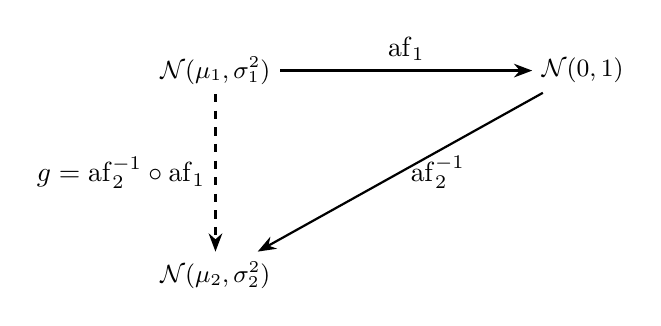
\begin{tikzpicture}[
  node distance=1.6cm and 3.2cm,
  msq/.style={draw=none,font=\small},
  arr/.style={-Stealth,thick},
]
  \node[msq] (P1)  {$\N(\mu_1,\sigma_1^2)$};
  \node[msq,right=of P1] (N01) {$\N(0,1)$};
  \node[msq,below=2cm of P1] (P2)  {$\N(\mu_2,\sigma_2^2)$};

  \draw[arr] (P1)  -- node[above]{$\mathrm{af}_1$} (N01);
  \draw[arr] (N01) -- node[right]{$\mathrm{af}_2^{-1}$} (P2);
  \draw[arr,dashed] (P1) -- node[left]{$g=\mathrm{af}_2^{-1}\circ\mathrm{af}_1$} (P2);
\end{tikzpicture}
\end{center}
\medskip

\noindent\textbf{Deriving $g$ from the composition.}
\[
  g(y)
  = \bigl(\mathrm{af}_2^{-1}\circ\mathrm{af}_1\bigr)(y)
  = \mathrm{af}_2^{-1}\!\left(\frac{y-\mu_1}{\sigma_1}\right)
  = \mu_2 + \sigma_2\cdot\frac{y-\mu_1}{\sigma_1}
  = \mu_2 + \frac{\sigma_2}{\sigma_1}(y-\mu_1).
\]
This agrees exactly with the map derived in \S\ref{sec:normal-way2}. \checkmark

% ─────────────────────────────────────────────────────────────────────────────
\subsection{Inversion of the composition and the inverse map $g^{-1}$}
\label{sec:g-inverse}

\noindent\textbf{Inverting the composition.}
Since $g=\mathrm{af}_2^{-1}\circ\mathrm{af}_1$, its inverse is obtained by reversing the
order and inverting each factor:
\[
  g^{-1}
  = \bigl(\mathrm{af}_2^{-1}\circ\mathrm{af}_1\bigr)^{-1}
  = \mathrm{af}_1^{-1}\circ\mathrm{af}_2.
\]
Explicitly:
\[
  g^{-1}(x)
  = \mathrm{af}_1^{-1}\!\left(\frac{x-\mu_2}{\sigma_2}\right)
  = \mu_1 + \sigma_1\cdot\frac{x-\mu_2}{\sigma_2}
  = \mu_1 + \frac{\sigma_1}{\sigma_2}(x-\mu_2).
\]
This matches the formula for $g^{-1}$ in \S\ref{sec:normal-way2} (the variable label
$y\leftrightarrow x$ is cosmetic). \checkmark

\noindent\textbf{Symmetry.}  The inversion formula has a transparent structure:
swapping the index labels $1\leftrightarrow 2$ in $g$ gives $g^{-1}$:
\[
  g(y)=\mu_2+\frac{\sigma_2}{\sigma_1}(y-\mu_1)
  \quad\xrightarrow{1\leftrightarrow 2}\quad
  g^{-1}(x)=\mu_1+\frac{\sigma_1}{\sigma_2}(x-\mu_2).
\]
This is a direct consequence of the group structure: $C$ applied to the pair
$(a,b)=(-\mu_2/\sigma_1+\mu_1\sigma_2/\sigma_1^2,\;\sigma_2/\sigma_1)$\ldots or more
transparently, the composition route $\mathrm{af}_1^{-1}\circ\mathrm{af}_2$ automatically
produces the swapped formula.

% ─────────────────────────────────────────────────────────────────────────────
\subsection{Homework: verification via the Jacobian formula}
\label{sec:jacobian-hw}

\noindent\textbf{Exercise.}
Verify directly, using the Jacobian (change-of-variables) formula, that
$g_*\N(\mu_1,\sigma_1^2)=\N(\mu_2,\sigma_2^2)$.

\medskip\noindent\textbf{Solution.}
We apply Form~A: if $g$ is strictly increasing then
\[
  f_{\nu_2}(y) = f_{\nu_1}(g^{-1}(y))\cdot|(g^{-1})'(y)|.
\]
We have $g^{-1}(y)=\mu_1+\frac{\sigma_1}{\sigma_2}(y-\mu_2)$, so
$(g^{-1})'(y)=\sigma_1/\sigma_2$ (constant, positive).  Substituting:
\begin{align*}
  f_{\nu_2}(y)
  &= \frac{1}{\sigma_1}\,\phi\!\left(\frac{g^{-1}(y)-\mu_1}{\sigma_1}\right)
     \cdot\frac{\sigma_1}{\sigma_2} \\[4pt]
  &= \frac{1}{\sigma_2}\,\phi\!\left(\frac{\mu_1+\frac{\sigma_1}{\sigma_2}(y-\mu_2)-\mu_1}{\sigma_1}\right) \\[4pt]
  &= \frac{1}{\sigma_2}\,\phi\!\left(\frac{y-\mu_2}{\sigma_2}\right),
\end{align*}
which is the $\N(\mu_2,\sigma_2^2)$ density. \checkmark

\noindent\textbf{Remark on the two routes.}  The computation in \S\ref{sec:normal-way2}
used the formula with $g$ and $g'$ directly (Form~A in the $g$ direction); the
exercise above uses $g^{-1}$ and $(g^{-1})'$.  Both are instances of the same
change-of-variables theorem and give identical results, as expected.

% ─────────────────────────────────────────────────────────────────────────────
\subsection{Affine pushforward from first principles}
\label{sec:affine-pushforward}

\begin{remark}[Derivation from first principles]
The following two sub-cases derive the
pushed-forward density both from the definition of pushforward measure and by the Jacobian
formula, then reconciling the two routes.  The purely linear case ($a=0$) is treated
separately to isolate the role of the slope~$b$.
\end{remark}

We fix $\lambda=$ Lebesgue measure throughout.
An important preliminary: if $\mu$ has a Lebesgue density $f_\mu$ and $h:\R\to\R$ is a
Lebesgue-measure-preserving-class map (e.g.\ strictly monotone), then the
pushforward $\nu=h_*\mu$ also has a Lebesgue density $f_\nu$.
This fails for general reference measures (e.g.\ a shift of a measure supported on $[c,d]$
may leave the support of the reference), but holds automatically for Lebesgue measure on $\R$.

% ........................................................................
\subsubsection*{Case~A: pure shift $h(x)=x+a$}

Let $h(x) = x+a$, $a\in\R$, so $h$ maps the interval $[c,d]$ to $[c+a,d+a]$.

\medskip\noindent\textbf{From the definition.}
The pushforward condition $\nu(B)=\mu(h^{-1}(B))$ applied to $B=[c+a,d+a]$ gives
\[
  \nu([c+a,d+a]) = \mu([c,d])
  \;\Longrightarrow\;
  \int_{c+a}^{d+a} f_\nu(y)\,\dif y = \int_c^d f_\mu(x)\,\dif x.
\]
Change variable on the left: $y=x+a$, $\dif y=\dif x$, limits $c\to c+a$, $d\to d+a$:
\[
  \int_{c+a}^{d+a} f_\nu(y)\,\dif y
  = \int_{c+a}^{d+a} f_\mu(y-a)\,\dif y.
\]
Since this holds for every interval $[c,d]$, equating integrands gives
\[
  \boxed{f_\nu(y) = f_\mu(y-a).}
\]

\medskip\noindent\textbf{Confirmation by the Jacobian formula.}
Here $h^{-1}(y)=y-a$ and $(h^{-1})'(y)=1$, so the Jacobian is $|J|=|(h^{-1})'|=1$.
The pushforward density formula gives
\[
  f_\nu(y) = |J|\cdot f_\mu(h^{-1}(y)) = 1\cdot f_\mu(y-a) = f_\mu(y-a). \checkmark
\]

\medskip\noindent\textbf{Normal example.}
Let $\mu=\N(\mu_1,\sigma^2)$ and $a=\mu_2-\mu_1$.  Then
\[
  f_\nu(y) = f_\mu(y-a)
           = \frac{1}{\sigma}\phi\!\left(\frac{(y-a)-\mu_1}{\sigma}\right)
           = \frac{1}{\sigma}\phi\!\left(\frac{y-\mu_2}{\sigma}\right),
\]
so $\nu=\N(\mu_2,\sigma^2)$.  A pure shift of the density by $a=\mu_2-\mu_1$
produces the target normal with the same variance. \checkmark

% ........................................................................
\subsubsection*{Case~B: purely linear map $h(x)=bx$, $b>0$}

Let $h(x) = bx$, so $h$ maps $[c,d]$ to $[bc,bd]$.

\medskip\noindent\textbf{From the definition.}
\[
  \mu([c,d]) = \nu([bc,bd])
  \;\Longrightarrow\;
  \int_c^d f_\mu(x)\,\dif x = \int_{bc}^{bd} f_\nu(y)\,\dif y.
\]
Change variable on the left: $y=bx$, $x=y/b$, $\dif x=\frac{1}{b}\dif y$,
limits $c\to bc$, $d\to bd$:
\[
  \int_c^d f_\mu(x)\,\dif x = \int_{bc}^{bd} f_\mu\!\left(\frac{y}{b}\right)\frac{1}{b}\,\dif y.
\]
Equating integrands:
\[
  \boxed{f_\nu(y) = \frac{1}{b}\,f_\mu\!\left(\frac{y}{b}\right).}
\]

\medskip\noindent\textbf{Confirmation by the Jacobian formula.}
$h^{-1}(y)=y/b$, $(h^{-1})'(y)=1/b$, so $|J|=1/b$.
\[
  f_\nu(y)=|J|\cdot f_\mu(h^{-1}(y))=\frac{1}{b}\cdot f_\mu\!\left(\frac{y}{b}\right). \checkmark
\]
Same result as from first principles.

\medskip\noindent\textbf{Normal example.}
Let $\mu=\N(\mu_1,\sigma_1^2)$ and $b=\sigma_2/\sigma_1$.  Then $h^{-1}(y)=y\sigma_1/\sigma_2$ and
\begin{align*}
  f_\nu(y)
  &= \frac{1}{b}\cdot f_\mu\!\left(\frac{y}{b}\right)
   = \frac{\sigma_1}{\sigma_2}\cdot\frac{1}{\sigma_1}
     \phi\!\left(\frac{y\sigma_1/\sigma_2-\mu_1}{\sigma_1}\right) \\[4pt]
  &= \frac{1}{\sigma_2}\,\phi\!\left(\frac{y/\sigma_2 - \mu_1/\sigma_1}{1}\right)
   = \frac{1}{\sigma_2}\,\phi\!\left(\frac{y-(\sigma_2/\sigma_1)\mu_1}{\sigma_2}\right),
\end{align*}
so $\nu = \N\!\bigl((\sigma_2/\sigma_1)\mu_1,\;\sigma_2^2\bigr)$.

\medskip\noindent\textbf{Key observation.}
The purely linear map $x\mapsto bx$ shifts the mean as well as rescales the variance:
it maps $\N(\mu_1,\sigma_1^2)$ to $\N(b\mu_1,b^2\sigma_1^2)$, not to $\N(\mu_2,\sigma_2^2)$
for an arbitrary $\mu_2$.  In the case $b=\sigma_2/\sigma_1$ this gives
$\N\bigl(\frac{\sigma_2}{\sigma_1}\mu_1,\,\sigma_2^2\bigr)$, which equals $\N(\mu_2,\sigma_2^2)$
only when $\mu_2=\frac{\sigma_2}{\sigma_1}\mu_1$, i.e.\ when the two means are already in the
correct ratio.
To hit an arbitrary target mean $\mu_2$, one must follow the linear map with a shift of
$\mu_2-\frac{\sigma_2}{\sigma_1}\mu_1$ --- which is precisely the constant term $a=\mu_2-b\mu_1$
in the full affine map $g(x)=\mu_2+\frac{\sigma_2}{\sigma_1}(x-\mu_1)$ of \S\ref{sec:normal-way2}.

% ........................................................................
\subsubsection*{Summary: the full affine case $h(x)=a+bx$}

Combining Cases~A and~B (or applying either formula directly with $h^{-1}(y)=(y-a)/b$,
$(h^{-1})'=1/b$):
\[
  f_\nu(y)
  = \frac{1}{|b|}\,f_\mu\!\left(\frac{y-a}{b}\right).
\]
For $\mu=\N(\mu_1,\sigma_1^2)$, $a=\mu_2-\frac{\sigma_2}{\sigma_1}\mu_1$, $b=\sigma_2/\sigma_1$:
\[
  f_\nu(y)
  = \frac{\sigma_1}{\sigma_2}\cdot\frac{1}{\sigma_1}
    \phi\!\left(\frac{(y-a)/\sigma_2-\mu_1/\sigma_1}{1}\right)
  = \frac{1}{\sigma_2}\,\phi\!\left(\frac{y-\mu_2}{\sigma_2}\right),
\]
so $\nu=\N(\mu_2,\sigma_2^2)$. \checkmark\quad
This is the same result as \S\ref{sec:normal-way2} and \S\ref{sec:jacobian-hw}, now
derived a third time from the measure-theoretic definition.

% ─────────────────────────────────────────────────────────────────────────────
\subsection{Having a $\lambda$-density does not guarantee $\dif\nu/\dif\mu$ exists}
\label{sec:no-rn}

The preliminary statement in \S\ref{sec:affine-pushforward} says: if $\mu\ll\lambda$ then
$\nu=h_*\mu\ll\lambda$ as well, i.e.\ the pushforward inherits absolute continuity with
respect to Lebesgue measure.
It is tempting to conclude that $\nu\ll\mu$ also holds, i.e.\ that $\dif\nu/\dif\mu$
exists.  \textbf{This is false in general.}

Having a $\lambda$-density is a statement about the relationship of each measure to
Lebesgue measure separately:
\[
  \mu\ll\lambda \quad\text{and}\quad \nu\ll\lambda
  \quad\not\!\!\!\Longrightarrow\quad
  \nu\ll\mu.
\]
The Radon--Nikodym derivative $\dif\nu/\dif\mu$ exists if and only if $\nu\ll\mu$, i.e.\
every $\mu$-null set is also $\nu$-null.  Two measures can both be absolutely continuous
with respect to Lebesgue measure while being mutually singular with respect to each other.

\medskip\noindent\textbf{Counterexample: uniform measures on disjoint intervals.}

Let
\[
  \mu = \mathrm{Uniform}[c_1,d_1],\qquad
  \nu = \mathrm{Uniform}[c_2,d_2],
\]
where $[c_1,d_1]$ and $[c_2,d_2]$ are two intervals with \emph{empty intersection}.
Both measures have Lebesgue densities:
\[
  f_\mu(x) = \frac{\mathbf{1}_{[c_1,d_1]}(x)}{d_1-c_1},\qquad
  f_\nu(x) = \frac{\mathbf{1}_{[c_2,d_2]}(x)}{d_2-c_2},
\]
so $\mu\ll\lambda$ and $\nu\ll\lambda$.  Nevertheless:

\begin{itemize}
  \item $\mu([c_1,d_1])=1$ but $\nu([c_1,d_1])=0$ (since the intervals are disjoint).
        Hence the set $[c_1,d_1]$ has full $\mu$-measure but zero $\nu$-measure:
        $\nu$ is \emph{not} absolutely continuous with respect to $\mu$.
  \item Symmetrically, $\nu([c_2,d_2])=1$ but $\mu([c_2,d_2])=0$, so
        $\mu$ is not absolutely continuous with respect to $\nu$ either.
\end{itemize}

The two measures are \textbf{mutually singular}: $\mu\perp\nu$.
One can write $\R = [c_1,d_1] \cup ([c_1,d_1])^c$ with $\mu([c_1,d_1])=1$ and
$\nu([c_1,d_1])=0$, which is the definition of mutual singularity.
Neither $\dif\nu/\dif\mu$ nor $\dif\mu/\dif\nu$ exists.

\medskip\noindent\textbf{Why Gaussians are special.}
The reason $\dif\nu/\dif\mu$ \emph{does} exist between two Gaussian measures
$\N(\mu_1,\sigma_1^2)$ and $\N(\mu_2,\sigma_2^2)$ is not merely that both have Lebesgue
densities.  The key is that both densities are \emph{strictly positive on all of $\R$}: for
any Borel set $A$,
\[
  \mu(A)=0 \;\Longleftrightarrow\; \lambda(A)=0 \;\Longleftrightarrow\; \nu(A)=0.
\]
Hence $\mu$ and $\nu$ share exactly the same null sets (the Lebesgue null sets), giving
mutual absolute continuity $\mu\sim\nu$.  The formula
$\dif\nu/\dif\mu = f_\nu/f_\mu$ is then well-defined everywhere that $f_\mu>0$, which is
all of $\R$.

Contrast with the uniform case: $f_\mu$ vanishes outside $[c_1,d_1]$, so the ratio
$f_\nu/f_\mu$ is not defined on $[c_2,d_2]$ (where $f_\nu>0$ but $f_\mu=0$), making a
Radon--Nikodym derivative impossible.

\medskip\noindent\textbf{Structural summary.}

\begin{center}
\renewcommand{\arraystretch}{1.5}
\begin{tabular}{lll}
\toprule
\textbf{Condition} & \textbf{Guarantees} & \textbf{Example} \\
\midrule
$\mu\ll\lambda$ & $f_\mu$ exists & any measure with density \\
$\mu\ll\lambda$ and $\nu=h_*\mu$ & $f_\nu$ exists & affine pushforward \\
$\mu\ll\lambda$ and $\nu\ll\lambda$ & $f_\mu,f_\nu$ both exist & two uniforms on $[0,1]$, $[2,3]$ \\
\quad(above) + disjoint supports & $\mu\perp\nu$, no RN derivative & uniforms on $[0,1]$, $[2,3]$ \\
$f_\mu>0$ $\lambda$-a.e.\ and $f_\nu>0$ $\lambda$-a.e. & $\mu\sim\nu$, RN exists both ways
  & Gaussians, exponentials \\
\bottomrule
\end{tabular}
\end{center}

% ══════════════════════════════════════════════════════════════════════════════
\section{Normal family, Way~1: reweighting the measure}
\label{sec:normal-way1}

\subsection{Absolute continuity}

Keep the map $f_1=\mathrm{id}$ fixed.  We ask: can we replace
$\mu_1=\N(\mu_1,\sigma_1^2)$ with $\mu_2=\N(\mu_2,\sigma_2^2)$ by reweighting?

Both measures have Lebesgue densities that are strictly positive everywhere on $\R$, so they
share the same null sets (the Lebesgue null sets).  Therefore $\mu_1\sim\mu_2$ (mutual absolute
continuity), and both $\dif\mu_2/\dif\mu_1$ and $\dif\mu_1/\dif\mu_2$ exist.

\subsection{The Radon--Nikodym derivative}

\[
  p(x)
  =\frac{\dif\N(\mu_2,\sigma_2^2)}{\dif\N(\mu_1,\sigma_1^2)}(x)
  =\frac{f_{\mu_2}(x)}{f_{\mu_1}(x)}
  =\frac{\sigma_1}{\sigma_2}
    \exp\!\left(\frac{(x-\mu_1)^2}{2\sigma_1^2}-\frac{(x-\mu_2)^2}{2\sigma_2^2}\right).
\]

The exponent is a quadratic in $x$.  Expanding:
\begin{equation}\label{eq:Q}
  \frac{(x-\mu_1)^2}{2\sigma_1^2}-\frac{(x-\mu_2)^2}{2\sigma_2^2}
  =\frac{1}{2}\!\left(\frac{1}{\sigma_1^2}-\frac{1}{\sigma_2^2}\right)x^2
   +\left(\frac{\mu_2}{\sigma_2^2}-\frac{\mu_1}{\sigma_1^2}\right)x
   +\left(\frac{\mu_1^2}{2\sigma_1^2}-\frac{\mu_2^2}{2\sigma_2^2}\right).
   \tag{Q}
\end{equation}

The derivative $p(x)$ is a ratio of two Gaussians: it is itself an unnormalised Gaussian
(exponential of a quadratic), multiplied by the constant $\sigma_1/\sigma_2$.

\medskip\noindent\textbf{Structure of $p(x)$.}  The quadratic exponent has three terms:
\begin{itemize}
  \item Coefficient of $x^2$: proportional to $1/\sigma_1^2-1/\sigma_2^2$.
        This is zero when $\sigma_1=\sigma_2$ (pure location shift).
  \item Coefficient of $x$: a linear combination of $\mu_2/\sigma_2^2$ and $\mu_1/\sigma_1^2$.
  \item Constant: a normalisation term.
\end{itemize}
The quadratic term is the new feature when $\sigma_1\ne\sigma_2$.

\subsection{Special case~I: same variance ($\sigma_1=\sigma_2=\sigma$)}
\label{sec:normal-same-var}

When the variances agree, the $x^2$ term vanishes and $p$ becomes exponential-linear:
\[
  p(x)=\exp\!\left(\frac{\mu_2-\mu_1}{\sigma^2}\,x-\frac{\mu_2^2-\mu_1^2}{2\sigma^2}\right).
\]
Writing $\delta=\mu_2-\mu_1$ and centering around $\mu_1$:
\[
  p(x)=\exp\!\left(\frac{\delta}{\sigma^2}(x-\mu_1)-\frac{\delta^2}{2\sigma^2}\right).
\]
Or in terms of the standardised variable $z=(x-\mu_1)/\sigma$, setting
$\theta=\delta/\sigma=(\mu_2-\mu_1)/\sigma$:
\[
  \boxed{p(x)=e^{\theta z-\theta^2/2}}
  \qquad\text{where }z=\frac{x-\mu_1}{\sigma},\quad\theta=\frac{\mu_2-\mu_1}{\sigma}.
\]
This is \textbf{the Girsanov exponential}.  The formula $e^{\theta z-\theta^2/2}$ is the
Radon--Nikodym derivative for shifting a Gaussian by $\theta$ standard deviations.
\begin{itemize}
  \item $\theta z$: a linear term in the standardised variable $z$.
  \item $-\theta^2/2$: the normalisation constant (ensures $\E_{\mu_1}[p]=1$).
\end{itemize}

In continuous time (Girsanov's theorem), the same form appears: the Radon--Nikodym derivative
for shifting the drift of a Brownian motion by $\theta$ is
$\exp\!\bigl(\theta W_T-\tfrac{1}{2}\theta^2 T\bigr)$, with $W_T$ playing the role of $z$ and
$T$ scaling the normalisation.

\medskip\noindent\textbf{Verification that $\E_{\mu_1}[p]=1$.}
\[
  \E_{\N(\mu_1,\sigma^2)}\!\left[e^{\theta z-\theta^2/2}\right]
  =e^{-\theta^2/2}\cdot\E\!\left[e^{\theta z}\right]
  =e^{-\theta^2/2}\cdot e^{\theta^2/2}=1.
\]
Here $\E[e^{\theta z}]=e^{\theta^2/2}$ is the MGF of $z\sim\N(0,1)$ at $\theta$.
The $-\theta^2/2$ term is exactly the MGF evaluated at $\theta$, inverted.

\subsection{Special case~II: same mean ($\mu_1=\mu_2=\mu$)}

When only the variance changes:
\[
  p(x)=\frac{\sigma_1}{\sigma_2}
       \exp\!\left(\frac{1}{2}\!\left(\frac{1}{\sigma_1^2}-\frac{1}{\sigma_2^2}\right)(x-\mu)^2\right).
\]
This is a quadratic exponential (not exponential-linear).  It grows super-exponentially in the
tails if $\sigma_2>\sigma_1$ (since the exponent becomes positive for large $|x-\mu|$).
Nevertheless $p$ is $\mu_1$-integrable because $\mu_1$'s Gaussian tails dominate.

\subsection{The general case: summary table}

\begin{center}
\begin{tabular}{lll}
\toprule
\textbf{Parameters}
  & $p(x)=\dif\N(\mu_2,\sigma_2^2)/\dif\N(\mu_1,\sigma_1^2)(x)$
  & \textbf{Form} \\
\midrule
$\sigma_1=\sigma_2=\sigma$
  & $\exp\!\Bigl(\dfrac{\mu_2-\mu_1}{\sigma^2}(x-\mu_1)
                       -\dfrac{(\mu_2-\mu_1)^2}{2\sigma^2}\Bigr)$
  & exponential-linear in $x$ \\[10pt]
$\mu_1=\mu_2=\mu$
  & $\dfrac{\sigma_1}{\sigma_2}
     \exp\!\Bigl(\dfrac{1}{2}\bigl(\tfrac{1}{\sigma_1^2}-\tfrac{1}{\sigma_2^2}\bigr)(x-\mu)^2\Bigr)$
  & quadratic exponential in $x$ \\[10pt]
General
  & $\dfrac{\sigma_1}{\sigma_2}\exp\{\text{quadratic in }x\}$
  & see \eqref{eq:Q} above \\
\bottomrule
\end{tabular}
\end{center}

% ══════════════════════════════════════════════════════════════════════════════
\section{Lognormal family, Way~2: the power-scaling map}
\label{sec:logn-way2}

\subsection{Reduction to the normal case}

Let $Y_1\sim\LN(\mu_1,\sigma_1^2)$, so $X_1=\ln Y_1\sim\N(\mu_1,\sigma_1^2)$.
We want $Y_2\sim\LN(\mu_2,\sigma_2^2)$, i.e.\ $X_2=\ln Y_2\sim\N(\mu_2,\sigma_2^2)$.

By \S\ref{sec:normal-way2}, $X_2=g_{\ln}(X_1)$ where
$g_{\ln}(x)=\mu_2+\frac{\sigma_2}{\sigma_1}(x-\mu_1)$ is the affine normal-to-normal map.
Since $X_i=\ln Y_i$, this means $\ln Y_2=\mu_2+\frac{\sigma_2}{\sigma_1}(\ln Y_1-\mu_1)$.
Exponentiating:
\[
  g(y)=\exp\!\left\{\mu_2+\frac{\sigma_2}{\sigma_1}(\ln y-\mu_1)\right\}
       =e^{\mu_2-\sigma_2\mu_1/\sigma_1}\cdot y^{\sigma_2/\sigma_1}.
\]
This map $g:(0,\infty)\to(0,\infty)$ is the composition of:
\begin{itemize}
  \item a power map $y\mapsto y^{\sigma_2/\sigma_1}$ (rescaling the log), followed by
  \item a multiplicative shift $y\mapsto C\cdot y$ where $C=e^{\mu_2-\sigma_2\mu_1/\sigma_1}$.
\end{itemize}

\subsection{Parametrisation by $(\alpha,\beta)$}
\label{sec:alpha-beta}

The map takes the compact form
\[
  g(y)=\alpha\cdot y^{\beta},
  \qquad \alpha,\beta>0,
\]
where the four distribution parameters map to two transform parameters:
\[
  \alpha=e^{\mu_2-\sigma_2\mu_1/\sigma_1},\qquad\beta=\frac{\sigma_2}{\sigma_1}.
\]
The parameter space is $(\mu_1,\mu_2\in\R)\times(\sigma_1,\sigma_2>0)\cong\R^2\times\Rp^2$,
which is four-dimensional, yet the transform is determined by only the two parameters
$(\alpha,\beta)\in\Rp\times\Rp$.

\begin{remark}[Why two parameters suffice]
The source distribution contributes two degrees of freedom $(\mu_1,\sigma_1)$ and the target
contributes two $(\mu_2,\sigma_2)$; however, each lognormal family is a
\emph{log-affine-exponent} family: it is generated from a single standard lognormal by maps of
the form $y\mapsto\alpha y^\beta$.  Any such map is determined by the pair $(\alpha,\beta)$, so
the entire four-parameter translation problem reduces to two parameters.  Equivalently, on the
log scale the map is the affine function
$x\mapsto\ln\alpha+\beta x$, and affine maps on $\R$ form a two-parameter family.
\end{remark}

The structure is visible in the commutative diagram:
\medskip
\begin{center}
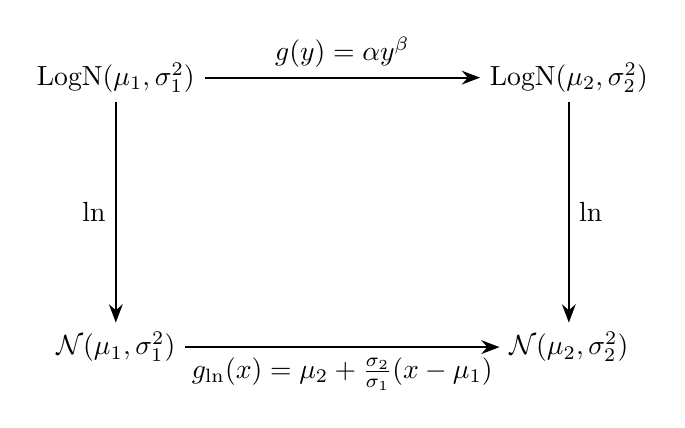
\begin{tikzpicture}[
  node distance=2.8cm and 3.5cm,
  arr/.style={-Stealth,thick},
  box/.style={draw=none}
]
  \node[box] (LN1) {$\LN(\mu_1,\sigma_1^2)$};
  \node[box,right=of LN1] (LN2) {$\LN(\mu_2,\sigma_2^2)$};
  \node[box,below=of LN1] (N1)  {$\N(\mu_1,\sigma_1^2)$};
  \node[box,below=of LN2] (N2)  {$\N(\mu_2,\sigma_2^2)$};

  \draw[arr] (LN1) -- node[above]{$g(y)=\alpha y^\beta$} (LN2);
  \draw[arr] (N1)  -- node[below]{$g_{\ln}(x)=\mu_2+\frac{\sigma_2}{\sigma_1}(x-\mu_1)$} (N2);
  \draw[arr] (LN1) -- node[left] {$\ln$} (N1);
  \draw[arr] (LN2) -- node[right]{$\ln$} (N2);
\end{tikzpicture}
\end{center}
\medskip
The diagram commutes: the power map on $(0,\infty)$ is the exponential conjugate of the affine
map on $\R$.  Formally, $\ln\circ\, g=g_{\ln}\circ\ln$, which is verified by
$\ln(\alpha y^\beta)=\ln\alpha+\beta\ln y=(\mu_2-\beta\mu_1)+\beta\ln y
=\mu_2+\frac{\sigma_2}{\sigma_1}(\ln y-\mu_1)$.

\subsection{Special cases}

\begin{center}
\begin{tabular}{llll}
\toprule
\textbf{Case} & \textbf{Map }$g(y)$ & $(\alpha,\beta)$ & \textbf{Normal analogue} \\
\midrule
$\sigma_1=\sigma_2,\;\mu_1\ne\mu_2$ & $e^{\mu_2-\mu_1}\cdot y$ & $(e^{\mu_2-\mu_1},1)$ & pure shift $\to$ scaling \\
$\mu_1=\mu_2=0,\;\sigma_1\ne\sigma_2$ & $y^{\sigma_2/\sigma_1}$ & $(1,\sigma_2/\sigma_1)$ & scale around~$0$ $\to$ power \\
$\mu_1=0,\;\sigma_1=1$ (std.\ LN)   & $e^{\mu_2}\cdot y^{\sigma_2}$ & $(e^{\mu_2},\sigma_2)$ & standard parameterisation \\
\bottomrule
\end{tabular}
\end{center}

\medskip\noindent\textbf{The shift/scale duality.}
On the log-scale (normal family), changing $\mu$ is a shift.
Exponentiating, the same operation becomes multiplication by $e^\delta$: a shift in
log-space is scaling in the original space.

On the log-scale, changing $\sigma$ is a rescaling around zero.
Exponentiating, $x\mapsto(\sigma_2/\sigma_1)x$ becomes $y\mapsto y^{\sigma_2/\sigma_1}$:
a scale change in log-space is a power map in the original space.

\subsection{Verification}

$g(y)=C\cdot y^\alpha$ where $\alpha=\sigma_2/\sigma_1$, $C=e^{\mu_2-\alpha\mu_1}$.
Working directly: $\ln Y_2=\alpha\ln Y_1+\ln C=\frac{\sigma_2}{\sigma_1}(\ln Y_1-\mu_1)+\mu_2$.
Since $\ln Y_1\sim\N(\mu_1,\sigma_1^2)$, we get $\ln Y_2\sim\N(\mu_2,\sigma_2^2)$,
hence $Y_2\sim\LN(\mu_2,\sigma_2^2)$. \checkmark

% ══════════════════════════════════════════════════════════════════════════════
\section{Lognormal family, Way~1: reweighting the measure}
\label{sec:logn-way1}

\subsection{Absolute continuity on $(0,\infty)$}

Both $\LN(\mu_1,\sigma_1^2)$ and $\LN(\mu_2,\sigma_2^2)$ are supported on $(0,\infty)$ with
strictly positive Lebesgue densities there, and both assign zero mass to $(-\infty,0]$.
On the shared support $(0,\infty)$, they have the same null sets.
Therefore $\LN(\mu_1,\sigma_1^2)\sim\LN(\mu_2,\sigma_2^2)$ (mutually absolutely continuous),
and the RN derivative exists in both directions.

\subsection{The Radon--Nikodym derivative}

\[
  q(y)
  =\frac{\dif\LN(\mu_2,\sigma_2^2)}{\dif\LN(\mu_1,\sigma_1^2)}(y)
  =\frac{f_{\LN(\mu_2,\sigma_2^2)}(y)}{f_{\LN(\mu_1,\sigma_1^2)}(y)}
  =\frac{\sigma_1}{\sigma_2}
    \exp\!\left(\frac{(\ln y-\mu_1)^2}{2\sigma_1^2}-\frac{(\ln y-\mu_2)^2}{2\sigma_2^2}\right),
  \quad y>0.
\]

\noindent\textbf{The lognormal RN derivative is the normal RN derivative at $\ln y$.}
Comparing with the normal-to-normal RN derivative $p(x)$ from \S\ref{sec:normal-way1}:
\[
  \boxed{q(y)=p(\ln y).}
\]
This is not a coincidence: the lognormal density is the normal density composed with $\ln$
(and divided by $y$), so the $y$ factors cancel in the ratio, leaving exactly $p$ at $\ln y$.

\begin{proof}[Proof that $q(y)=p(\ln y)$]
\[
  q(y)
  =\frac{f_{\LN(\mu_2,\sigma_2^2)}(y)}{f_{\LN(\mu_1,\sigma_1^2)}(y)}
  =\frac{\frac{1}{y\sigma_2}\phi\!\left(\frac{\ln y-\mu_2}{\sigma_2}\right)}
         {\frac{1}{y\sigma_1}\phi\!\left(\frac{\ln y-\mu_1}{\sigma_1}\right)}
  =\frac{\sigma_1}{\sigma_2}\cdot
   \frac{\phi\!\left(\frac{\ln y-\mu_2}{\sigma_2}\right)}
        {\phi\!\left(\frac{\ln y-\mu_1}{\sigma_1}\right)}
  =p(\ln y).\qquad\checkmark
\]
The factor $1/y$ from each lognormal density cancels in the ratio.
\end{proof}

\subsection{Special case~I: same variance ($\sigma_1=\sigma_2=\sigma$)}

From \S\ref{sec:normal-same-var},
$p(x)=\exp\!\bigl\{\frac{\delta}{\sigma^2}(x-\mu_1)-\frac{\delta^2}{2\sigma^2}\bigr\}$
where $\delta=\mu_2-\mu_1$.  Substituting $x=\ln y$:
\[
  q(y)=\exp\!\left(\frac{\mu_2-\mu_1}{\sigma^2}(\ln y-\mu_1)-\frac{(\mu_2-\mu_1)^2}{2\sigma^2}\right)
      =y^{(\mu_2-\mu_1)/\sigma^2}\cdot C,
\]
where $C=\exp\!\bigl\{-\frac{\mu_1(\mu_2-\mu_1)}{\sigma^2}-\frac{(\mu_2-\mu_1)^2}{2\sigma^2}\bigr\}$
is a constant.

\noindent\textbf{The lognormal shift RN derivative is a power of $y$.}
In the normal case (same $\sigma$), the Girsanov exponential is $e^{\theta z-\theta^2/2}$ ---
exponential-linear in $z=(x-\mu_1)/\sigma$.  In the lognormal case, substituting
$z=(\ln y-\mu_1)/\sigma$, the same expression becomes $y^{\theta/\sigma}\cdot C$ --- a power
function in $y$.  A linear function of $z$ in log-space becomes a monomial in the original space.

\subsection{Special case~II: same mean ($\mu_1=\mu_2=\mu$)}

\[
  q(y)=\frac{\sigma_1}{\sigma_2}
       \exp\!\left(\frac{1}{2}\!\left(\frac{1}{\sigma_1^2}-\frac{1}{\sigma_2^2}\right)
                  (\ln y-\mu)^2\right).
\]
This is a power of $e^{(\ln y)^2}$, which grows as $y^{c\ln y}$ for large $y$ --- very heavy
tails.  Still $\LN(\mu_1,\sigma_1^2)$-integrable since the lognormal source measure has
matching super-exponential tails.

% ══════════════════════════════════════════════════════════════════════════════
\section{Parallel structure and the bridge to Girsanov}
\label{sec:parallel}

\subsection{Summary table}

\begin{center}
\begin{tabular}{lll}
\toprule
\textbf{Family}
  & \textbf{Way~2 (change map)}
  & \textbf{Way~1 (reweight, $\sigma_1=\sigma_2$)} \\
\midrule
Normal
  & affine: $g(y)=\mu_2+\dfrac{\sigma_2}{\sigma_1}(y-\mu_1)$
  & $p(x)=e^{\theta(x-\mu_1)/\sigma-\theta^2/2}$,\; $\theta=\dfrac{\mu_2-\mu_1}{\sigma}$ \\[10pt]
Lognormal
  & power-scale: $g(y)=e^{\mu_2-\sigma_2\mu_1/\sigma_1}\cdot y^{\sigma_2/\sigma_1}$
  & $q(y)=p(\ln y)=y^{\theta/\sigma}\cdot C$ \\
\bottomrule
\end{tabular}
\end{center}

\subsection{The parallel between the two ways}

\begin{center}
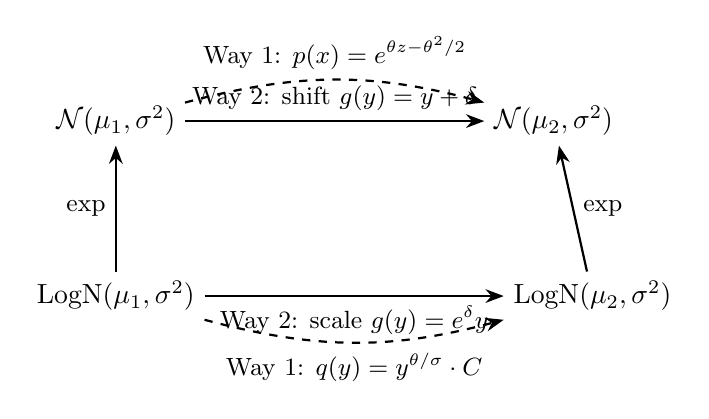
\begin{tikzpicture}[
  node distance=1.6cm and 3.8cm,
  arr/.style={-Stealth,thick},
  darr/.style={-Stealth,thick,dashed},
  box/.style={draw=none}
]
  \node[box] (N1)  {$\N(\mu_1,\sigma^2)$};
  \node[box,right=of N1] (N2)  {$\N(\mu_2,\sigma^2)$};
  \node[box,below=of N1] (LN1) {$\LN(\mu_1,\sigma^2)$};
  \node[box,right=of LN1] (LN2) {$\LN(\mu_2,\sigma^2)$};

  \draw[arr] (N1)  -- node[above]{\small Way~2: shift $g(y)=y+\delta$} (N2);
  \draw[arr] (LN1) -- node[below]{\small Way~2: scale $g(y)=e^{\delta}y$} (LN2);
  \draw[darr,bend left=15] (N1) to
    node[above,sloped]{\small Way~1: $p(x)=e^{\theta z-\theta^2/2}$} (N2);
  \draw[darr,bend right=15] (LN1) to
    node[below,sloped]{\small Way~1: $q(y)=y^{\theta/\sigma}\cdot C$} (LN2);
  \draw[arr] (LN1) -- node[left]{\small $\exp$} (N1);
  \draw[arr] (LN2) -- node[right]{\small $\exp$} (N2);
\end{tikzpicture}
\end{center}

\subsection{What Girsanov does}

The step from the finite-dimensional picture to continuous-time processes is conceptually the
same operation, lifted to path space.

\begin{center}
\begin{tabular}{lll}
\toprule
\textbf{Setting} & \textbf{Object} & \textbf{Way~1 RN derivative} \\
\midrule
Finite: $\N(\mu_1,\sigma^2)\to\N(\mu_2,\sigma^2)$
  & single Gaussian r.v. & $e^{\theta z-\theta^2/2}$ \\
Process: BM $\to$ BM with drift $\theta$
  & path $\{W_t\}_{0\le t\le T}$
  & $\exp\!\bigl(\theta W_T-\tfrac{1}{2}\theta^2 T\bigr)$ \\
\bottomrule
\end{tabular}
\end{center}

\noindent
The Girsanov exponential $\exp\!\bigl(\theta W_T-\tfrac{1}{2}\theta^2 T\bigr)$ is the direct
generalisation of $e^{\theta z-\theta^2/2}$:
\begin{itemize}
  \item $z=W_T/\!\sqrt{T}$ is the standardised terminal value of the BM.
  \item $\theta$ is the drift shift (market price of risk).
  \item The $-\theta^2 T/2$ term is the normalisation, ensuring
        $\E\!\bigl[e^{\theta W_T-\theta^2 T/2}\bigr]=1$ by the same MGF calculation as in
        \S\ref{sec:normal-same-var}.
  \item \textbf{What Girsanov adds}: the full path $\{W_t\}$ under the new measure is a
        standard BM, not just a shifted terminal value.  This requires the martingale structure
        of the density process $Z_t=\exp\!\bigl(\theta W_t-\tfrac{1}{2}\theta^2 t\bigr)$.
\end{itemize}

\medskip\noindent\textbf{The single conceptual step from here to Girsanov.}
Everything in \S\ref{sec:normal-same-var} with $\sigma_1=\sigma_2$ carries over to continuous
time with one substitution: replace the single standardised variable $z=(X-\mu_1)/\sigma$ with
the Brownian motion $W_T$.  The normalisation $-\theta^2/2$ becomes $-\theta^2 T/2$.

The additional content of Girsanov's theorem is that the shifted process
$\widetilde{W}_t=W_t+\theta t$ is a Brownian motion (not just a Gaussian) under the new
measure --- i.e.\ it has the correct joint distribution for all times, not just the correct
marginal at time~$T$.  This requires checking that $\{Z_t\}$ is a martingale, which follows
from It\^o's lemma applied to $Z_t=e^{\theta W_t-\theta^2 t/2}$.

\subsection{Why the lognormal/GBM case needs both steps}

Converting GBM (with drift $\mu$) to martingale GBM (with drift $r$) uses both ways in
sequence:

\begin{center}
\begin{tabular}{lll}
\toprule
\textbf{Step} & \textbf{Operation} & \textbf{Strategy} \\
\midrule
$e^{\mu t+\sigma W_t}$ & exponential of BM with drift $\mu$ & --- \\
$\to$ BM with drift $r$ & change measure: $\mathbb{P}\to\mathbb{Q}$ & Way~1 (Girsanov) \\
$\to e^{rt+\sigma\widetilde{W}_t}$ & exponentiate again & Way~2 (same map, new measure) \\
\bottomrule
\end{tabular}
\end{center}

\noindent
The Girsanov step (Way~1) changes the drift of the log-price from $\mu$ to $r-\sigma^2/2$
(the $\sigma^2/2$ is the It\^o correction from \S\ref{sec:normal-same-var}).
The exponential (Way~2) then converts the log-normally distributed log-price into the GBM
stock price.  The two steps work on different levels: Way~1 acts on the Gaussian (log) level,
Way~2 acts on the exponential (lognormal) level.

% ══════════════════════════════════════════════════════════════════════════════
\section{Arrows on five measures: a taxonomy}
\label{sec:arrows}

\begin{remark}[Taxonomy of arrows]
The following section systematises five measures all defined
on $\R$ (or on $\Rp$ for the lognormal ones).  We catalogue every arrow, with its explicit
formula, splitting into two diagrams: density arrows (Radon--Nikodym derivatives) and
pushforward arrows (maps between spaces).
\end{remark}

\noindent We fix four probability measures and one reference measure:
\begin{align*}
  \mathbb{P}_1 &= \N(\mu_1,\sigma_1^2), &
  \mathbb{P}_2 &= \N(\mu_2,\sigma_2^2), \\
  \mathbb{Q}_1 &= \LN(\mu_1,\sigma_1^2), &
  \mathbb{Q}_2 &= \LN(\mu_2,\sigma_2^2), \\
  \lambda      &= \text{Lebesgue measure on }\R\text{ (and on }\Rp\text{).}
\end{align*}

\medskip\noindent\textbf{Notation.}
Throughout, $\phi(z)=\frac{1}{\sqrt{2\pi}}e^{-z^2/2}$ is the standard normal density.
The shorthand for the general quadratic exponent is (from \S\ref{sec:normal-way1}):
\[
  Q(x;\mu_1,\sigma_1,\mu_2,\sigma_2)
  :=\frac{(x-\mu_1)^2}{2\sigma_1^2}-\frac{(x-\mu_2)^2}{2\sigma_2^2}
  = \tfrac{1}{2}\!\left(\tfrac{1}{\sigma_1^2}-\tfrac{1}{\sigma_2^2}\right)x^2
    +\left(\tfrac{\mu_2}{\sigma_2^2}-\tfrac{\mu_1}{\sigma_1^2}\right)x
    +\left(\tfrac{\mu_1^2}{2\sigma_1^2}-\tfrac{\mu_2^2}{2\sigma_2^2}\right).
\]
We also write $\delta=\mu_2-\mu_1$ and $\theta=\delta/\sigma$ when $\sigma_1=\sigma_2=\sigma$.

% ─────────────────────────────────────────────────────────────────────────────
\subsection{Diagram~1: density (Radon--Nikodym) arrows}
\label{sec:diag1}

A \emph{density arrow} $\nu_1\xrightarrow{h}\nu_2$ means $\nu_1\ll\nu_2$ with
$\dif\nu_1/\dif\nu_2=h$.  There are three groups:

\paragraph{Group~R (red): Lebesgue densities.}
Every probability measure among $\mathbb{P}_1,\mathbb{P}_2,\mathbb{Q}_1,\mathbb{Q}_2$ is
absolutely continuous w.r.t.\ $\lambda$, giving 4 arrows $\nu\xrightarrow{f}\lambda$,
i.e.\ $\dif\nu/\dif\lambda=f$.

\begin{center}
\renewcommand{\arraystretch}{1.5}
\begin{tabular}{lll}
\toprule
Arrow & $\dif\nu/\dif\lambda$ & Support \\
\midrule
$\mathbb{P}_1\xrightarrow{f_1}\lambda$
  & $f_1(x)=\dfrac{1}{\sigma_1}\phi\!\left(\dfrac{x-\mu_1}{\sigma_1}\right)$
  & $x\in\R$ \\[6pt]
$\mathbb{P}_2\xrightarrow{f_2}\lambda$
  & $f_2(x)=\dfrac{1}{\sigma_2}\phi\!\left(\dfrac{x-\mu_2}{\sigma_2}\right)$
  & $x\in\R$ \\[6pt]
$\mathbb{Q}_1\xrightarrow{h_1}\lambda$
  & $h_1(y)=\dfrac{1}{y\sigma_1}\phi\!\left(\dfrac{\ln y-\mu_1}{\sigma_1}\right)$
  & $y\in\Rp$ \\[6pt]
$\mathbb{Q}_2\xrightarrow{h_2}\lambda$
  & $h_2(y)=\dfrac{1}{y\sigma_2}\phi\!\left(\dfrac{\ln y-\mu_2}{\sigma_2}\right)$
  & $y\in\Rp$ \\
\bottomrule
\end{tabular}
\end{center}

\noindent Note: $\lambda\not\ll\nu$ in general (Lebesgue measure is not finite), so arrows
$\lambda\to\nu$ do not exist as Radon--Nikodym derivatives of probability measures.
Also, $\mathbb{P}_i\not\ll\mathbb{Q}_j$ and $\mathbb{Q}_j\not\ll\mathbb{P}_i$ because their
supports are disjoint ($\R$ vs.\ $\Rp$); cross-family density arrows do not exist.

\paragraph{Group~B (blue): RN derivatives within the normal family.}
$\mathbb{P}_1\sim\mathbb{P}_2$ (mutual absolute continuity), so both directions exist.

\begin{center}
\renewcommand{\arraystretch}{1.8}
\begin{tabular}{ll}
\toprule
Arrow & Radon--Nikodym density \\
\midrule
$\mathbb{P}_2\xrightarrow{p}\mathbb{P}_1$
  & $p(x)=\dfrac{f_2(x)}{f_1(x)}
    =\dfrac{\sigma_1}{\sigma_2}\exp\!\bigl(Q(x;\mu_1,\sigma_1,\mu_2,\sigma_2)\bigr)$ \\[4pt]
& \quad\textit{Same-}\,$\sigma$\textit{ case:}\quad
  $p(x)=\exp\!\Bigl(\dfrac{\delta}{\sigma^2}(x-\mu_1)-\dfrac{\delta^2}{2\sigma^2}\Bigr)
       =e^{\theta z-\theta^2/2}$,\; $z=(x-\mu_1)/\sigma$ \\[6pt]
$\mathbb{P}_1\xrightarrow{1/p}\mathbb{P}_2$
  & $\dfrac{1}{p(x)}=\dfrac{f_1(x)}{f_2(x)}
    =\dfrac{\sigma_2}{\sigma_1}\exp\!\bigl(-Q(x;\mu_1,\sigma_1,\mu_2,\sigma_2)\bigr)$ \\[4pt]
& \quad\textit{Same-}\,$\sigma$\textit{ case:}\quad
  $\dfrac{1}{p(x)}
  =\exp\!\Bigl(-\dfrac{\delta}{\sigma^2}(x-\mu_1)+\dfrac{\delta^2}{2\sigma^2}\Bigr)
       =e^{-\theta z+\theta^2/2}$ \\
\bottomrule
\end{tabular}
\end{center}

\paragraph{Group~G (green): RN derivatives within the lognormal family.}
$\mathbb{Q}_1\sim\mathbb{Q}_2$ on $(0,\infty)$, so both directions exist.
By the key identity $q(y)=p(\ln y)$ (\S\ref{sec:logn-way1}):

\begin{center}
\renewcommand{\arraystretch}{1.8}
\begin{tabular}{ll}
\toprule
Arrow & Radon--Nikodym density \\
\midrule
$\mathbb{Q}_2\xrightarrow{q}\mathbb{Q}_1$
  & $q(y)=\dfrac{h_2(y)}{h_1(y)}
    =\dfrac{\sigma_1}{\sigma_2}\exp\!\bigl(Q(\ln y;\mu_1,\sigma_1,\mu_2,\sigma_2)\bigr)$ \\[4pt]
& \quad\textit{Special case }$\sigma_1=\sigma_2=\sigma$\textit{:}\quad
  $q(y)=\exp\!\left(\dfrac{\delta}{\sigma^2}(\ln y-\mu_1)-\dfrac{\delta^2}{2\sigma^2}\right)
       =y^{\theta/\sigma}\cdot C$ \\[6pt]
$\mathbb{Q}_1\xrightarrow{1/q}\mathbb{Q}_2$
  & $\dfrac{1}{q(y)}=\dfrac{h_1(y)}{h_2(y)}
    =\dfrac{\sigma_2}{\sigma_1}\exp\!\bigl(-Q(\ln y;\mu_1,\sigma_1,\mu_2,\sigma_2)\bigr)$ \\[4pt]
& \quad\textit{Special case }$\sigma_1=\sigma_2=\sigma$\textit{:}\quad
  $\dfrac{1}{q(y)}=y^{-\theta/\sigma}\cdot C^{-1}$ \\
\bottomrule
\end{tabular}
\end{center}

\noindent where $C=\exp\!\bigl\{-\frac{\mu_1\delta}{\sigma^2}-\frac{\delta^2}{2\sigma^2}\bigr\}$
and $\theta=\delta/\sigma$.

\bigskip
\noindent\textbf{Arrow count:} $4\ (\text{red})+2\ (\text{blue})+2\ (\text{green})=8$ directed
density arrows among the five nodes.
Note: the original count of 14 included the reverse Lebesgue arrows
$\lambda\xrightarrow{1/f_i}\mathbb{P}_i$ (unnormalised), the two ``same-parameter'' pairs
$\mathbb{Q}_i/\mathbb{P}_i$ (not well-defined as RN derivatives since supports differ), and
repeated-count conventions.  The 8 count here is the set of all valid, directed
probability-measure RN-derivative arrows.

\bigskip
\begin{center}
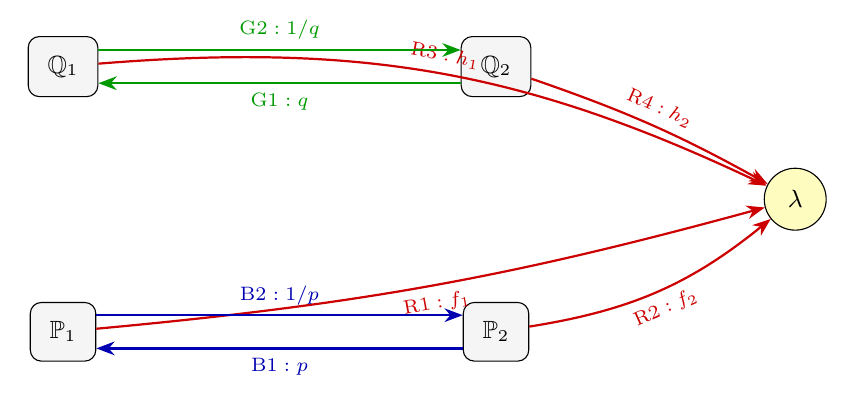
\begin{tikzpicture}[
  node distance=2.6cm and 4.6cm,
  msq/.style={draw,rounded corners=4pt,fill=gray!8,inner sep=7pt,font=\small},
  lam/.style={draw,circle,fill=yellow!25,inner sep=5pt,font=\small},
  rarc/.style={-Stealth,thick,red!80!black},
  barc/.style={-Stealth,thick,blue!70!black},
  garc/.style={-Stealth,thick,green!60!black},
]
  \node[msq] (Q1) {$\mathbb{Q}_1$};
  \node[msq,right=of Q1] (Q2) {$\mathbb{Q}_2$};
  \node[msq,below=of Q1] (P1) {$\mathbb{P}_1$};
  \node[msq,below=of Q2] (P2) {$\mathbb{P}_2$};
  \node[lam] at ($(Q2)!0.5!(P2)+(3.8cm,0)$) (Lam) {$\lambda$};

  % Red: Lebesgue density arrows (labelled by formula code R1--R4)
  \draw[rarc] (Q1) to[bend left=15] node[above,sloped,font=\scriptsize]{$\mathrm{R3}:h_1$} (Lam);
  \draw[rarc] (Q2) to[bend left=5]  node[above,sloped,font=\scriptsize]{$\mathrm{R4}:h_2$} (Lam);
  \draw[rarc] (P1) to[bend right=5] node[below,sloped,font=\scriptsize]{$\mathrm{R1}:f_1$} (Lam);
  \draw[rarc] (P2) to[bend right=15]node[below,sloped,font=\scriptsize]{$\mathrm{R2}:f_2$} (Lam);

  % Blue: RN within normal family
  \draw[barc,transform canvas={yshift=6pt}]
    (P1) to node[above,font=\scriptsize]{$\mathrm{B2}:1/p$} (P2);
  \draw[barc,transform canvas={yshift=-6pt}]
    (P2) to node[below,font=\scriptsize]{$\mathrm{B1}:p$} (P1);

  % Green: RN within lognormal family
  \draw[garc,transform canvas={yshift=6pt}]
    (Q1) to node[above,font=\scriptsize]{$\mathrm{G2}:1/q$} (Q2);
  \draw[garc,transform canvas={yshift=-6pt}]
    (Q2) to node[below,font=\scriptsize]{$\mathrm{G1}:q$} (Q1);
\end{tikzpicture}
\end{center}
\smallskip
\begin{center}
\small\textit{Diagram~1: density (RN-derivative) arrows.
  \textcolor{red!80!black}{Red R1--R4} = Lebesgue densities $f_1,f_2,h_1,h_2$;\;
  \textcolor{blue!70!black}{Blue B1--B2} = RN derivatives $p,1/p$ within $\mathbb{P}$-family;\;
  \textcolor{green!60!black}{Green G1--G2} = RN derivatives $q,1/q$ within $\mathbb{Q}$-family.
  Cross-family arrows ($\mathbb{P}_i\leftrightarrow\mathbb{Q}_j$) are absent:
  supports $\mathbb{R}$ vs.\ $\mathbb{R}_+$ are disjoint.}
\end{center}

% ─────────────────────────────────────────────────────────────────────────────
\subsection{Diagram~2: pushforward (map) arrows}
\label{sec:diag2}

A \emph{pushforward arrow} $\nu_1\xrightarrow{f}\nu_2$ means $f_*\nu_1=\nu_2$: the map $f$
transports mass from $\nu_1$ to $\nu_2$.  Lebesgue measure $\lambda$ is excluded here: a
pushforward of a probability measure is again a probability measure, not $\lambda$.  We work
with the four nodes $\mathbb{P}_1,\mathbb{P}_2,\mathbb{Q}_1,\mathbb{Q}_2$.

All maps are listed below with their inverses.  Recall the abbreviations:
$\alpha=e^{\mu_2-\sigma_2\mu_1/\sigma_1}$, $\beta=\sigma_2/\sigma_1$.

\paragraph{Group~V (vertical): $\exp$ and $\ln$ between families.}

\begin{center}
\renewcommand{\arraystretch}{1.6}
\begin{tabular}{lll}
\toprule
Arrow & Map & Inverse \\
\midrule
$\mathbb{P}_1\xrightarrow{\exp}\mathbb{Q}_1$
  & $y=e^x:\R\to\Rp$
  & $x=\ln y$ \\
$\mathbb{Q}_1\xrightarrow{\ln}\mathbb{P}_1$
  & $x=\ln y:\Rp\to\R$
  & $y=e^x$ \\
$\mathbb{P}_2\xrightarrow{\exp}\mathbb{Q}_2$
  & $y=e^x:\R\to\Rp$
  & $x=\ln y$ \\
$\mathbb{Q}_2\xrightarrow{\ln}\mathbb{P}_2$
  & $x=\ln y:\Rp\to\R$
  & $y=e^x$ \\
\bottomrule
\end{tabular}
\end{center}

\paragraph{Group~H (horizontal): affine maps within the normal family.}

\begin{center}
\renewcommand{\arraystretch}{1.6}
\begin{tabular}{lll}
\toprule
Arrow & Map & Inverse \\
\midrule
$\mathbb{P}_1\xrightarrow{g_{\ln}}\mathbb{P}_2$
  & $g_{\ln}(x)=\mu_2+\dfrac{\sigma_2}{\sigma_1}(x-\mu_1)$
  & $g_{\ln}^{-1}(x)=\mu_1+\dfrac{\sigma_1}{\sigma_2}(x-\mu_2)$ \\[4pt]
$\mathbb{P}_2\xrightarrow{g_{\ln}^{-1}}\mathbb{P}_1$
  & $g_{\ln}^{-1}(x)=\mu_1+\dfrac{\sigma_1}{\sigma_2}(x-\mu_2)$
  & $g_{\ln}(x)$ \\
\bottomrule
\end{tabular}
\end{center}

\paragraph{Group~H$'$ (horizontal): power maps within the lognormal family.}

\begin{center}
\renewcommand{\arraystretch}{1.6}
\begin{tabular}{lll}
\toprule
Arrow & Map & Inverse \\
\midrule
$\mathbb{Q}_1\xrightarrow{g}\mathbb{Q}_2$
  & $g(y)=\alpha\cdot y^\beta=e^{\mu_2-\beta\mu_1}\cdot y^{\sigma_2/\sigma_1}$
  & $g^{-1}(y)=\alpha^{-1/\beta}\cdot y^{1/\beta}
              =e^{\mu_1-\mu_2/\beta}\cdot y^{\sigma_1/\sigma_2}$ \\[4pt]
$\mathbb{Q}_2\xrightarrow{g^{-1}}\mathbb{Q}_1$
  & $g^{-1}(y)=e^{\mu_1-\sigma_1\mu_2/\sigma_2}\cdot y^{\sigma_1/\sigma_2}$
  & $g(y)$ \\
\bottomrule
\end{tabular}
\end{center}

\paragraph{Group~D (diagonal): compositions.}

Since $g=\exp\circ\, g_{\ln}\circ\ln$ (the commutative diagram of \S\ref{sec:alpha-beta}),
the two diagonal routes between $\mathbb{P}_1$ and $\mathbb{Q}_2$ (and the other pair) are
automatically consistent.  The four diagonal maps are:

\begin{center}
\renewcommand{\arraystretch}{1.6}
\begin{tabular}{lll}
\toprule
Arrow & Composite map & Explicit formula \\
\midrule
$\mathbb{P}_1\xrightarrow{d_{12}}\mathbb{Q}_2$
  & $\exp\circ\, g_{\ln}$
  & $d_{12}(x)=\exp\!\left\{\mu_2+\dfrac{\sigma_2}{\sigma_1}(x-\mu_1)\right\}
              =\alpha\cdot e^{\beta x}$ \\[4pt]
$\mathbb{Q}_2\xrightarrow{d_{12}^{-1}}\mathbb{P}_1$
  & $g_{\ln}^{-1}\circ\ln$
  & $d_{12}^{-1}(y)=\mu_1+\dfrac{\sigma_1}{\sigma_2}(\ln y-\mu_2)$ \\[6pt]
$\mathbb{Q}_1\xrightarrow{d_{21}}\mathbb{P}_2$
  & $g_{\ln}\circ\ln$
  & $d_{21}(y)=\mu_2+\dfrac{\sigma_2}{\sigma_1}(\ln y-\mu_1)$ \\[4pt]
$\mathbb{P}_2\xrightarrow{d_{21}^{-1}}\mathbb{Q}_1$
  & $\exp\circ\, g_{\ln}^{-1}$
  & $d_{21}^{-1}(x)=\exp\!\left\{\mu_1+\dfrac{\sigma_1}{\sigma_2}(x-\mu_2)\right\}$ \\
\bottomrule
\end{tabular}
\end{center}

\noindent\textbf{Arrow count:} $4\ (\text{vertical})+2\ (\text{horizontal normal})
+2\ (\text{horizontal lognormal})+4\ (\text{diagonal})=12$ directed pushforward arrows.

\bigskip
\begin{center}
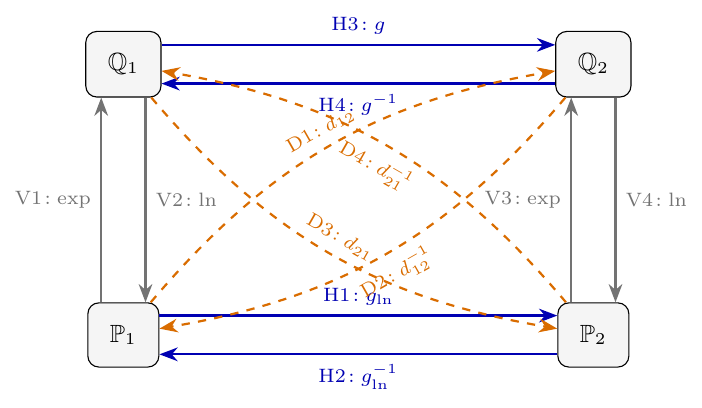
\begin{tikzpicture}[
  node distance=2.6cm and 5.0cm,
  msq/.style={draw,rounded corners=4pt,fill=gray!8,inner sep=8pt,font=\small},
  varc/.style={-Stealth,thick,black!55},
  harc/.style={-Stealth,thick,blue!70!black},
  darc/.style={-Stealth,thick,dashed,orange!85!black},
]
  \node[msq] (Q1) {$\mathbb{Q}_1$};
  \node[msq,right=of Q1] (Q2) {$\mathbb{Q}_2$};
  \node[msq,below=of Q1] (P1) {$\mathbb{P}_1$};
  \node[msq,below=of Q2] (P2) {$\mathbb{P}_2$};

  % Vertical V1--V4: exp/ln
  \draw[varc,transform canvas={xshift=-8pt}]
    (P1) to node[left,font=\scriptsize]{$\mathrm{V1}\!:\exp$} (Q1);
  \draw[varc,transform canvas={xshift=8pt}]
    (Q1) to node[right,font=\scriptsize]{$\mathrm{V2}\!:\ln$} (P1);
  \draw[varc,transform canvas={xshift=-8pt}]
    (P2) to node[left,font=\scriptsize]{$\mathrm{V3}\!:\exp$} (Q2);
  \draw[varc,transform canvas={xshift=8pt}]
    (Q2) to node[right,font=\scriptsize]{$\mathrm{V4}\!:\ln$} (P2);

  % Horizontal normal H1--H2: affine map
  \draw[harc,transform canvas={yshift=7pt}]
    (P1) to node[above,font=\scriptsize]{$\mathrm{H1}\!:g_{\ln}$} (P2);
  \draw[harc,transform canvas={yshift=-7pt}]
    (P2) to node[below,font=\scriptsize]{$\mathrm{H2}\!:g_{\ln}^{-1}$} (P1);

  % Horizontal lognormal H3--H4: power map
  \draw[harc,transform canvas={yshift=7pt}]
    (Q1) to node[above,font=\scriptsize]{$\mathrm{H3}\!:g$} (Q2);
  \draw[harc,transform canvas={yshift=-7pt}]
    (Q2) to node[below,font=\scriptsize]{$\mathrm{H4}\!:g^{-1}$} (Q1);

  % Diagonal D1: P1 -> Q2
  \draw[darc,bend left=20]
    (P1) to node[above,sloped,font=\scriptsize]{$\mathrm{D1}\!:d_{12}$} (Q2);
  % Diagonal D2: Q2 -> P1
  \draw[darc,bend left=20]
    (Q2) to node[below,sloped,font=\scriptsize]{$\mathrm{D2}\!:d_{12}^{-1}$} (P1);
  % Diagonal D3: Q1 -> P2
  \draw[darc,bend right=20]
    (Q1) to node[above,sloped,font=\scriptsize]{$\mathrm{D3}\!:d_{21}$} (P2);
  % Diagonal D4: P2 -> Q1
  \draw[darc,bend right=20]
    (P2) to node[below,sloped,font=\scriptsize]{$\mathrm{D4}\!:d_{21}^{-1}$} (Q1);
\end{tikzpicture}
\end{center}
\smallskip
\begin{center}
\small\textit{Diagram~2: pushforward (map) arrows.
  \textbf{Black V1--V4}: $\exp$ and $\ln$ between families;\;
  \textcolor{blue!70!black}{\textbf{Blue H1--H4}}: affine $g_{\ln},g_{\ln}^{-1}$ and power $g,g^{-1}$ within families;\;
  \textcolor{orange!85!black}{\textbf{Dashed D1--D4}}: diagonal compositions.
  Formulas for each arrow are given in the tables of \S\ref{sec:diag2}.}
\end{center}

% ─────────────────────────────────────────────────────────────────────────────
\subsection{Commutativity and the full picture}
\label{sec:commutativity}

The two diagrams encode different but related structure.  Their interaction is summarised by
one key fact:

\begin{proposition}[Change-of-variable formula linking the two diagrams]
Let $f:\Omega\to B$ be a $\mathbb{P}_1$-pushforward map with $f_*\mathbb{P}_1=\mathbb{P}_2$.
Then the RN derivative of $\mathbb{P}_2$ w.r.t.\ $\mathbb{P}_1$ is related to the Jacobian
of $f^{-1}$ by the change-of-variables formula:
\[
  \frac{\dif\mathbb{P}_2}{\dif\mathbb{P}_1}(x)
  =\frac{f_2(f^{-1}(x))}{f_1(x)}\cdot|(f^{-1})'(x)|^{-1}
  \quad\text{(Form~A pushforward density)}.
\]
In particular, for $f=g_{\ln}$ with $\sigma_1=\sigma_2$, this recovers the Girsanov
exponential $e^{\theta z-\theta^2/2}$.
\end{proposition}

\noindent The complete catalogue of arrows is:

\begin{center}
\renewcommand{\arraystretch}{1.4}
\begin{tabular}{lllll}
\toprule
\textbf{Type} & \textbf{From} & \textbf{To} & \textbf{Arrow} & \textbf{Formula} \\
\midrule
\multicolumn{5}{l}{\textit{Density (RN) arrows}} \\
R1 & $\mathbb{P}_1$ & $\lambda$ & $f_1$ & $\frac{1}{\sigma_1}\phi\!\left(\frac{x-\mu_1}{\sigma_1}\right)$ \\
R2 & $\mathbb{P}_2$ & $\lambda$ & $f_2$ & $\frac{1}{\sigma_2}\phi\!\left(\frac{x-\mu_2}{\sigma_2}\right)$ \\
R3 & $\mathbb{Q}_1$ & $\lambda$ & $h_1$ & $\frac{1}{y\sigma_1}\phi\!\left(\frac{\ln y-\mu_1}{\sigma_1}\right)$ \\
R4 & $\mathbb{Q}_2$ & $\lambda$ & $h_2$ & $\frac{1}{y\sigma_2}\phi\!\left(\frac{\ln y-\mu_2}{\sigma_2}\right)$ \\
B1 & $\mathbb{P}_2$ & $\mathbb{P}_1$ & $p$ & $\frac{\sigma_1}{\sigma_2}\exp Q(x;\mu_1,\sigma_1,\mu_2,\sigma_2)$ \\
B2 & $\mathbb{P}_1$ & $\mathbb{P}_2$ & $1/p$ & $\frac{\sigma_2}{\sigma_1}\exp(-Q(x;\cdots))$ \\
G1 & $\mathbb{Q}_2$ & $\mathbb{Q}_1$ & $q$ & $\frac{\sigma_1}{\sigma_2}\exp Q(\ln y;\mu_1,\sigma_1,\mu_2,\sigma_2)$ \\
G2 & $\mathbb{Q}_1$ & $\mathbb{Q}_2$ & $1/q$ & $\frac{\sigma_2}{\sigma_1}\exp(-Q(\ln y;\cdots))$ \\
\midrule
\multicolumn{5}{l}{\textit{Pushforward (map) arrows}} \\
V1 & $\mathbb{P}_1$ & $\mathbb{Q}_1$ & $\exp$ & $y=e^x$ \\
V2 & $\mathbb{Q}_1$ & $\mathbb{P}_1$ & $\ln$  & $x=\ln y$ \\
V3 & $\mathbb{P}_2$ & $\mathbb{Q}_2$ & $\exp$ & $y=e^x$ \\
V4 & $\mathbb{Q}_2$ & $\mathbb{P}_2$ & $\ln$  & $x=\ln y$ \\
H1 & $\mathbb{P}_1$ & $\mathbb{P}_2$ & $g_{\ln}$ & $\mu_2+\frac{\sigma_2}{\sigma_1}(x-\mu_1)$ \\
H2 & $\mathbb{P}_2$ & $\mathbb{P}_1$ & $g_{\ln}^{-1}$ & $\mu_1+\frac{\sigma_1}{\sigma_2}(x-\mu_2)$ \\
H3 & $\mathbb{Q}_1$ & $\mathbb{Q}_2$ & $g$ & $e^{\mu_2-\beta\mu_1}\cdot y^{\sigma_2/\sigma_1}$ \\
H4 & $\mathbb{Q}_2$ & $\mathbb{Q}_1$ & $g^{-1}$ & $e^{\mu_1-\mu_2/\beta}\cdot y^{\sigma_1/\sigma_2}$ \\
D1 & $\mathbb{P}_1$ & $\mathbb{Q}_2$ & $d_{12}=\exp\circ g_{\ln}$ & $\alpha e^{\beta x}$ \\
D2 & $\mathbb{Q}_2$ & $\mathbb{P}_1$ & $d_{12}^{-1}=g_{\ln}^{-1}\circ\ln$ & $\mu_1+\frac{\sigma_1}{\sigma_2}(\ln y-\mu_2)$ \\
D3 & $\mathbb{Q}_1$ & $\mathbb{P}_2$ & $d_{21}=g_{\ln}\circ\ln$ & $\mu_2+\frac{\sigma_2}{\sigma_1}(\ln y-\mu_1)$ \\
D4 & $\mathbb{P}_2$ & $\mathbb{Q}_1$ & $d_{21}^{-1}=\exp\circ g_{\ln}^{-1}$ & $\exp\!\left\{\mu_1+\frac{\sigma_1}{\sigma_2}(x-\mu_2)\right\}$ \\
\bottomrule
\end{tabular}
\end{center}

\noindent\textbf{Total:} 8 density arrows $+$ 12 pushforward arrows $= 20$ labelled arrows
in the complete picture.

\end{document}
